\chapter{Experiments}
We now delve into out contribution to tackling the problem of automatic differential diagnosis of Mendelian diseases. At this scope we have prepared a tailored KG integrated with patient data, that we describe in \Cref{sec:patientKG}. We then outline the approach used for link prediction, motivating the choice of hyperbolic graph representation learning techniques (\Cref{sec:linkPredictionDiffDiagnosis}). 

\section{Patient KG}\label{sec:patientKG}
In this section we describe the data that we have chosen for the task of differential diagnosis of Mendelian diseases. We proceed by exploring the underlying biomedical knowledge graph that we have used and the patient data that we have selected. We also describe how these data sources have been integrated into a single knowledge graph.

\subsection{Underlying biomedical KG}
Initially we have considered PrimeKG \cite{chandak2023PrimeKG}, a knowledge graph targeted at precision medicine analyses aggregating 20 high quality resources. Unfortunately, at the moment of use we have encountered substantial shortcomings in the representation of Mendelian diseases. Taking inspiration from the entities represented in PrimeKG, we have constructed a tailored knowledge graph. We have resorted to \emph{PheKnowLator} (\emph{Phenotype Knowledge Translator})~\cite{callahan2020PheKnowlator}\footnote{The Python library is available at \url{https://github.com/callahantiff/PheKnowLator}}, a KG framework designed for optimized construction of semantically-rich, large-scale biomedical KGs accounting for different standardized terminologies or vocabularies. 




with PheKnowLator \& type choice

\begin{figure}
    \centering
    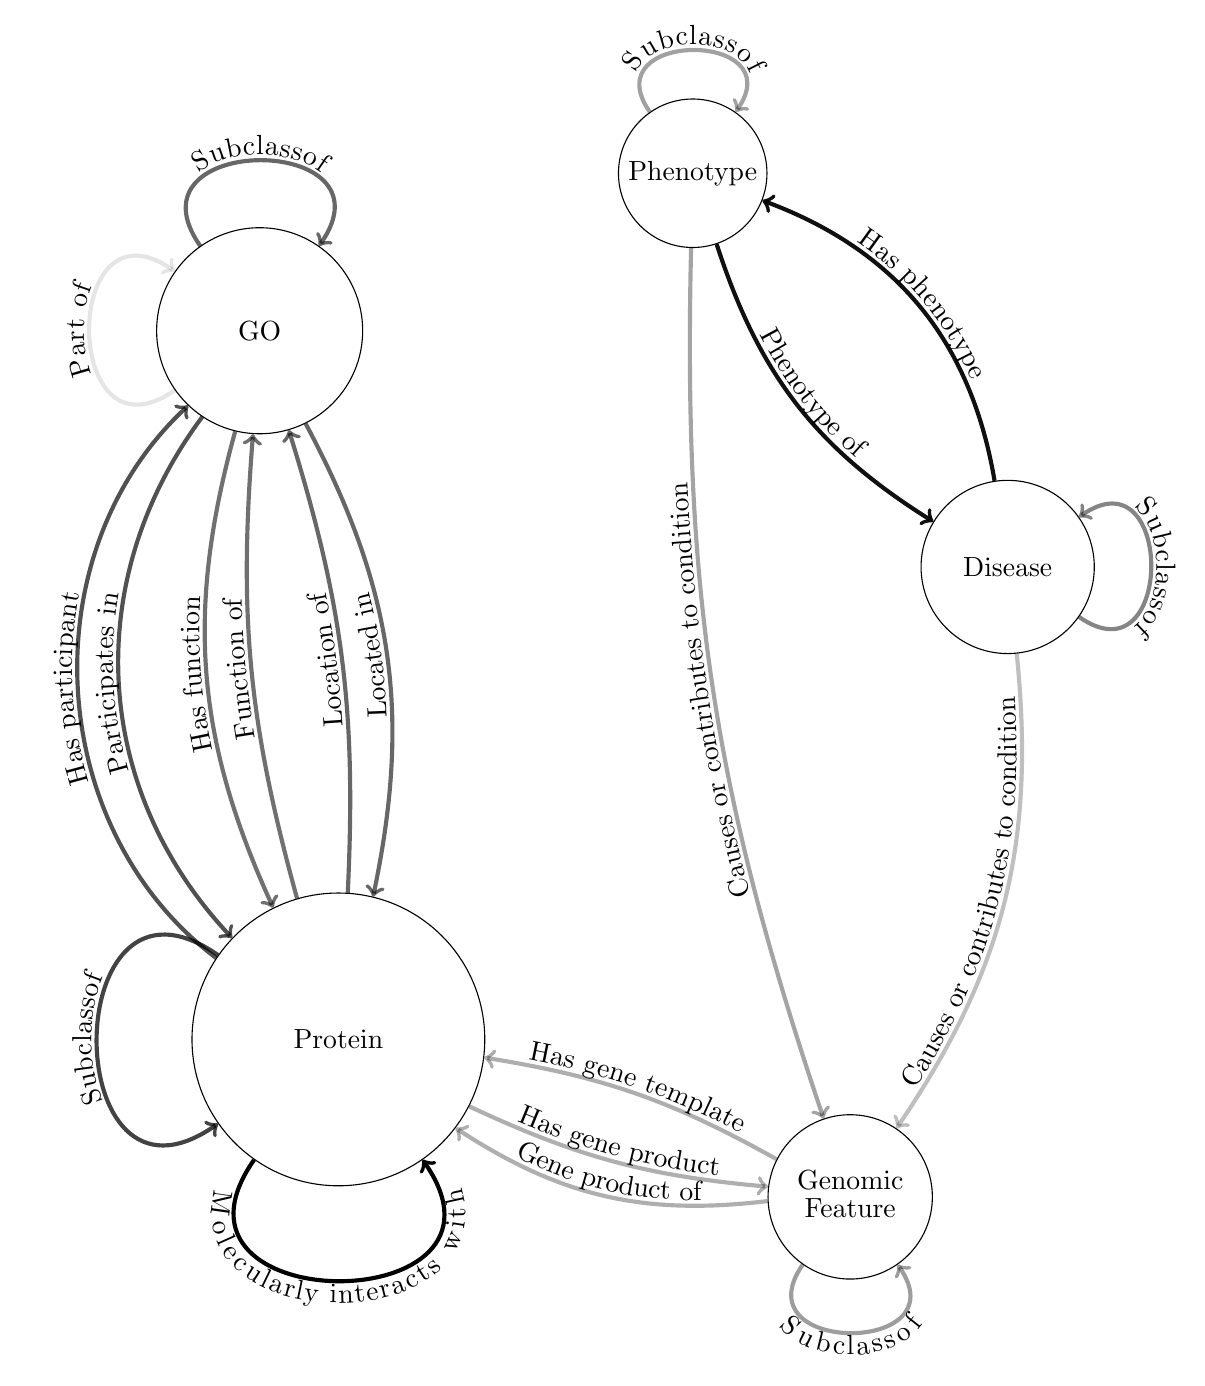
\begin{tikzpicture}
    \usetikzlibrary{decorations.text}

    \begin{scope}[xshift=1cm]
        % Nodes
        \node[circle, draw, fill=none, minimum size=3.718cm, inner sep=0pt] (Protein) at (-4,-3) {Protein};
        \node[circle, draw, fill=none, minimum size=2.617cm, inner sep=0pt] (GO) at (-5,6) {GO};
        \node[circle, draw, fill=none, minimum size=2.200cm, inner sep=0pt] (Disease) at (4.5,3) {Disease};
        \node[circle, draw, fill=none, minimum size=2.087cm, inner sep=0pt] (GenomicFeature) at (2.5,-5) {\begin{tabular}{c}Genomic\\[-0.5ex]Feature\end{tabular}};
        \node[circle, draw, fill=none, minimum size=1.886cm, inner sep=0pt] (Phenotype) at (0.5,8) {Phenotype};

        % Edges with curved labels
            \draw[->, line width=1.5pt, opacity=0.937927] (Disease) to[bend right=30] (Phenotype);
            \path[decorate, decoration={text along path, text align=center, raise=2pt, text={Has phenotype}}] (Phenotype) to[bend left=30] (Disease);

            \draw[->, line width=1.5pt, opacity=1.000000] (Protein) to[out=235, in=305, looseness=3] (Protein);
            \path[decorate, decoration={text along path, text align=center, raise=-8pt, text={Molecularly interacts with}}] (Protein) to[out=235, in=305, looseness=3](Protein);

            \draw[->, line width=1.5pt, opacity=0.478617] (Disease) to[out=-35, in=35, looseness=3] (Disease);
            \path[decorate, decoration={text along path, text align=center, raise=2pt, text={Subclassof}}] (Disease) to[out=35, in=-35, looseness=3] (Disease);

            \draw[->, line width=1.5pt, opacity=0.596164] (GO) to[out=125, in=55, looseness=3] (GO);
            \path[decorate, decoration={text along path, text align=center, raise=2pt, text={Subclassof}}] (GO) to[out=125, in=55, looseness=3] (GO);

            \draw[->, line width=1.5pt, opacity=0.383857] (GenomicFeature) to[out=235, in=305, looseness=3] (GenomicFeature);
            \path[decorate, decoration={text along path, text align=center, raise=-8pt, text={Subclassof}}] (GenomicFeature) to[out=235, in=305, looseness=3] (GenomicFeature);

            \draw[->, line width=1.5pt, opacity=0.367024] (Phenotype) to[out=125, in=55, looseness=3] (Phenotype);
            \path[decorate, decoration={text along path, text align=center, raise=2pt, text={Subclassof}}] (Phenotype) to[out=125, in=55, looseness=3] (Phenotype);

            \draw[->, line width=1.5pt, opacity=0.735558] (Protein) to[out=145, in=215, looseness=3] (Protein);
            \path[decorate, decoration={text along path, text align=center, raise=2pt, text={Subclassof}}] (Protein) to[out=215, in=145, looseness=3] (Protein);

            \draw[->, line width=1.5pt, opacity=0.561965] (Protein) to[bend left=10] (GO);
            \path[decorate, decoration={text along path, text align=center, raise=2pt, text={Function of}}] (Protein) to[bend left=10] (GO);


            \draw[->, line width=1.5pt, opacity=0.937927] (Phenotype) to[bend right=20] (Disease);
            \path[decorate, decoration={text along path, text align=center, raise=2pt, text={Phenotype of}}] (Phenotype) to[bend right=20] (Disease);

            \draw[->, line width=1.5pt, opacity=0.316749] (GenomicFeature) to[bend right=10] (Protein);
            \path[decorate, decoration={text along path, text align=center, raise=2pt, text={Has gene template}}] (Protein) to[bend left=10] (GenomicFeature);

            \draw[->, line width=1.5pt, opacity=0.561965] (GO) to[bend right=20] (Protein);
            \path[decorate, decoration={text along path, text align=center, raise=2pt, text={Has function}}] (Protein) to[bend left=20] (GO);

            \draw[->, line width=1.5pt, opacity=0.681528] (Protein) to[bend left=50] (GO);
            \path[decorate, decoration={text along path, text align=center, raise=2pt, text={Has participant}}] (Protein) to[bend left=50] (GO);

            \draw[->, line width=1.5pt, opacity=0.311908] (Protein) to[bend right=10] (GenomicFeature);
            \path[decorate, decoration={text along path, text align=center, raise=2pt, text={Has gene product}}] (Protein) to[bend right=10] (GenomicFeature);

           

            \draw[->, line width=1.5pt, opacity=0.595817] (Protein) to[bend right=10] (GO);
            \path[decorate, decoration={text along path, text align=center, raise=2pt, text={Location of}}] (Protein) to[bend right=10] (GO);

            \draw[->, line width=1.5pt, opacity=0.595822] (GO) to[bend left=20] (Protein);
            \path[decorate, decoration={text along path, text align=center, raise=2pt, text={Located in}}] (Protein) to[bend right=20] (GO);

            \draw[->, line width=1.5pt, opacity=0.681523] (GO) to[bend right=40] (Protein);
            \path[decorate, decoration={text along path, text align=center, raise=2pt, text={Participates in}}] (Protein) to[bend left=40] (GO);

            \draw[->, line width=1.5pt, opacity=0.250632] (Disease) to[bend left=20] (GenomicFeature);
            \path[decorate, decoration={text along path, text align=center, raise=2pt, text={Causes or contributes to condition}}] (GenomicFeature) to[bend right=20] (Disease);

            \draw[->, line width=1.5pt, opacity=0.356471] (Phenotype) to[bend right=10] (GenomicFeature);
            \path[decorate, decoration={text along path, text align=center, raise=2pt, text={Causes or contributes to condition}}] (GenomicFeature) to[bend left=10] (Phenotype);

            \draw[->, line width=1.5pt, opacity=0.311908] (GenomicFeature) to[bend left=20] (Protein);
            \path[decorate, decoration={text along path, text align=center, raise=2pt, text={Gene product of}}] (Protein) to[bend right=20] (GenomicFeature);

            \draw[->, line width=1.5pt, opacity=0.100000] (GO) to[out=215, in=145, looseness=3] (GO);
            \path[decorate, decoration={text along path, text align=center, raise=2pt, text={Part of}}] (GO) to[out=215, in=145, looseness=3] (GO);   \end{scope}
    \end{tikzpicture}

    \caption{A hypergraph representation of the underlying knowledge graph, having hypernodes representing the possibile node types and hyperedges for the most frequent edge predicates. The hypernodes' size and the hyperedges' opacity are logarithmic in the amount of node types and edge predicates respectively.}
    \label{fig:kg_hypergraph}
\end{figure}

\subsection{Patient data}
Phenopackets \& field choice

\subsection{Data integration}

\begin{figure}
    \centering
    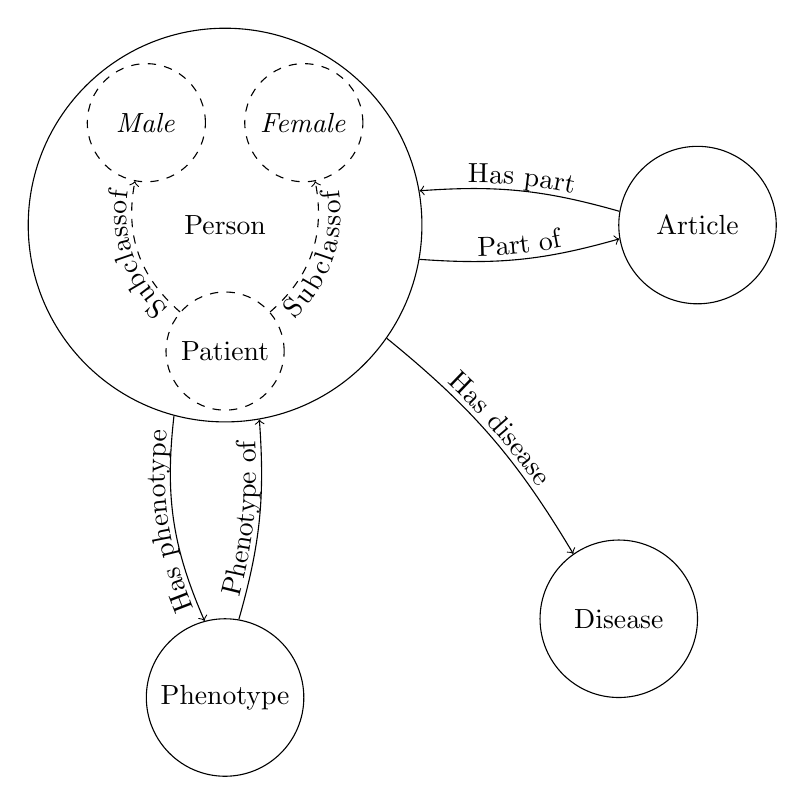
\begin{tikzpicture}
        % Nodes
        \node[circle, draw, fill=none, minimum size=2cm, inner sep=0pt] (Disease) at (1,4) {Disease};
        \node[circle, draw, fill=none, minimum size=2cm, inner sep=0pt] (Phenotype) at (-4,3) {Phenotype};
        \node[circle, draw, fill=none, minimum size=2cm, inner sep=0pt] (Article) at (2,9) {Article};
        \node[circle, draw, fill=none, minimum size=5cm, inner sep=0pt] (Person) at (-4,9) {Person};
        \node[circle, draw, dashed,  fill=none, minimum size=1.5cm, inner sep=0pt] (Male) at (-5,10.3) {\textit{Male}};
        \node[circle, draw, dashed, fill=none, minimum size=1.5cm, inner sep=0pt] (Female) at (-3,10.3) {\textit{Female}};
        \node[circle, draw, dashed, fill=none, minimum size=1.5cm, inner sep=0pt] (Patient) at (-4,7.4) {Patient};

        % Edges with curved labels
            \draw[->] (Person) to[bend right=10] (Article);
            \path[decorate, decoration={text along path, text align=center, raise=2pt, text={Part of}}] (Person) to[bend right=10] (Article);

            \draw[->] (Article) to[bend right=10] (Person);
            \path[decorate, decoration={text along path, text align=center, raise=2pt, text={Has part}}] (Person) to[bend left=10] (Article);

            \draw[dashed, ->] (Patient) to[bend left=30] (Male);
            \path[decorate, decoration={text along path, text align=center, raise=2pt, text={Subclassof}}] (Patient) to[bend left=30] (Male);
            \draw[dashed, ->] (Patient) to[bend right=30] (Female);
            \path[decorate, decoration={text along path, text align=center, raise=-8pt, text={Subclassof}}] (Patient) to[bend right=30] (Female);

            \draw[->] (Person) to[bend left=10] (Disease);
            \path[decorate, decoration={text along path, text align=center, raise=2pt, text={Has disease}}] (Person) to[bend left=10] (Disease);

            \draw[->] (Person) to[bend right=15] (Phenotype);
            \path[decorate, decoration={text along path, text align=center, raise=2pt, text={Has phenotype}}] (Phenotype) to[bend left=15] (Person);
            \draw[->] (Phenotype) to[bend right=10] (Person);
            \path[decorate, decoration={text along path, text align=center, raise=2pt, text={Phenotype of}}] (Phenotype) to[bend right=10] (Person);
    \end{tikzpicture}

    \caption{The hypergraph representing the node types and edge predicates added during the integration of the underlying knowledge graph and patient data. The nodes contained in the Person hypernode and the relative hyperedges are merely a semantic schematization of the data. In particular Male and Female correspond to single nodes in the knowledge graph.}
    \label{fig:patient_kg_hypergraph}
\end{figure}

\section{Link prediction for differential diagnosis}\label{sec:linkPredictionDiffDiagnosis}

\subsection{Why hyperbolic graph representation learning?}

\subsection{Experiment setup}
